\documentclass[12pt,english]{article}
\usepackage{mathptmx}

\usepackage{color}
\usepackage[dvipsnames]{xcolor}
\definecolor{darkblue}{RGB}{0.,0.,139.}

\usepackage[top=1in, bottom=1in, left=1in, right=1in]{geometry}

\usepackage{amsmath}
\usepackage{amstext}
\usepackage{amssymb}
\usepackage{setspace}
\usepackage{lipsum}

\usepackage[authoryear]{natbib}
\usepackage{url}
\usepackage{booktabs}
\usepackage[flushleft]{threeparttable}
\usepackage{graphicx}
\usepackage[english]{babel}
\usepackage{pdflscape}
\usepackage[unicode=true,pdfusetitle,
 bookmarks=true,bookmarksnumbered=false,bookmarksopen=false,
 breaklinks=true,pdfborder={0 0 0},backref=false,
 colorlinks,citecolor=black,filecolor=black,
 linkcolor=black,urlcolor=black]
 {hyperref}
\usepackage[all]{hypcap} % Links point to top of image, builds on hyperref
\usepackage{breakurl}    % Allows urls to wrap, including hyperref

\linespread{2}

\begin{document}

\begin{singlespace}
\title{Random Forest Machine Learning Prediction of Baseball Hall of Fame Induction}
\end{singlespace}

\author{Beth Felkner\thanks{Department of Economics, University of Oklahoma.\
E-mail~address:~\href{mailto:student.name@ou.edu}{bethfelkner@ou.edu}}}

% \date{\today}
\date{April 28, 2024}

\maketitle

\begin{abstract}
\begin{singlespace}
This project seeks to predict induction into the Baseball Hall of Fame classes of 2025-2028 by using a random forest algorithm for binary classification. I train the algorithm on the Hall of Fame ballot data from 2015-2024. With my optimized model, I achieve a predictive accuracy of 84\% on the test data. Predicted results for 2025-2028 are largely in line with what baseball analysts except, with the notable exception being that my model does not predict Ichiro Suzuki to be inducted. While the results are encouraging, the model could be strengthened by the inclusion of more predictor variables and a larger dataset. The primary implication of this research is that HoF induction can be predicted with a high degree of accuracy using solely baseball performance metrics, and thus claims that the HoF is rigged (like somebase fans like to make) are largely unsubstantiated. There is also a further implication about the many potential applications of machine learning in baseball and how teams could use advanced predictive analysis to change the future of the game. 
\end{singlespace}

\end{abstract}
\vfill{}

\pagebreak{}


\section{Introduction}\label{sec:intro}
I've been a huge baseball fan since I was 11 years old and watching nearly every Texas Rangers game is one of my most favorite past times, so naturally I knew I wanted to do something related to baseball for this project. As big of a Rangers fan as I am, however, I am perhaps an even bigger fan of all the statistics and metrics associated with baseball. Detailed statistics are kept for almost every baseball outcome imaginable, from Batting Average (BA or AVG) to walks to Earned Run Average (ERA) and everything in between. In addition to these "baseline" statistics, today's MLB statscape also includes a plethora of complex constructed metrics such as Wins Above Replacement (WAR) and On-Base Plus Slugging Plus (OPS+) which are designed to capture the overall value of a player to their team. And though it's not one of the metrics that will be included in my algorithms, I would be remiss to write a paper about baseball without mentioning the glorious and officially recognized by the MLB metric of the TOOTBLAN, which stands for Thrown Out On The Bases Like a Nincompoop. All this to say, the game of baseball includes a LOT of statistics.

For this paper, I wanted to focus on a particular baseball outcome that is often not well understood: election to the Baseball Hall of Fame (HoF). Players are considered eligible for the HoF and automatically added to the ballot if they played in the MLB for at least 10 full seasons and have been retired for at least five full seasons. To be elected, they must receive a vote from 75\% of ballot voters. If a player is not elected in their first year, they are eligible to remain on the ballot for up to 9 additional years so long as they received 5\% of votes in the preceding year. After 10 years they will be removed from the ballot and considered no longer eligible. 

Obviously, players are elected based on some combination of their performance across variables baseball metrics. However, some baseball have questioned the validity of HoF induction, suggesting it may be "rigged" or based on factors outside of baseball performance. For this project, I used a random forest machine learning model to predict the HoF status of a player based on their performance across a number of offensive metrics, in order to see how accurately HoF status could be predicted solely by baseball performance metrics.

\section{Literature Review}\label{sec:litreview}
Several previous researchers have attempted to predict Baseball Hall of Fame induction using random forests and other machine learning models. \cite{mills2011} use BBWAA (Baseball Writers' Association of America, the group that votes on the HoF ballots) data from 1950 to 2009. Their optimized model for hitters has an error rate of 2.6\%. Interestingly, their model predicted both Barry Bonds and Roger Clemens to make the HoF, both of whom have now exhausted their eligibility without making the ballot, both due to PED scandals. As will be discussed later, my model incurred a similar phenomenon with predicting Alex Rodriguez. \cite{mills2011} also analyzed whether racial discrimination was a factor in BBWAA voting, but did not find evidence that worthy players were excluded base on race. This is an intersting consideration, however, in line with some baseball fans believing the HoF is rigged.

\cite{freiman2010} also employed a random forest predictve model, but further refined his results by using a simulating annealing method. He ran several different forest models and to counter for the inherent randomness of predictor selection in a random forest model, he fed the results of each forest model into a logistic regression to produce final probability estimates. His best model had an out-of-sample prediction accuracy of approximately 75\%. He did note that his trying and discarding of many different models creates potentials concerns about overfitting. Similarly, \cite{smith2009} used data from players who had retired between 1950 and 2002. He used a Radial Basis Function to build separate models for hitters and pitchers. For pitchers, his model correctly predicted 21 out of 24 HoF inductions, while for batters his model corrected predicted 38 out of 45. 

\cite{young2008} employed an artificial neural network model. In addition to offensive metrics for position players, they also include fielding metrics and awards received (such as Gold Glove or Silver Slugger) as predictor variables. Their model using k-means reduction achieved prediction of 98\%. They also ran a logistic regression with the same predictor variables a baseline, and reported that their neural net prediction accuracy was 6\% higher than that of their baseline regression. Besides just HoF prediction, machine learning models have been applied towards many other outcomes/questions in baseball. \cite{koseler2018} provide a systematic literature review of existing baseball research which employs machine learning techniques. Applications discussed mentioned include predicting a pitcher's next pitch type based on previous pitches, predicting the winner of particular of a matchup between particular teams, predicting the probability of a strikeout given a particular batter and pitcher, and many more. 

In summary, there is an extensive body of literature about machine learning for baseball prediction generally. The body of literature specifically surrounding predction of HoF induction is much smaller, and notably, most of the research is about 15 years old. I think novel research on this question is warranted because both relative levels of baseball metrics and the HoF eligibility criteria have changed over the past 15 years. 


\section{Data}\label{sec:data}
I am using Hall of Fame Voting data from baseball-reference.com for the years 2015-2014. The datasets are published for each year on baseball-reference.com and include all players who became ballot eligible for that ballot year (meaning all players who played for at least 10 seasons and had been retired for five years as of that ballot year.) As a note, I had some confusion while I was compiling my data about if the baseball-reference.com datasets included all eligible players in each year or just a subset. I started with the baseball-reference data, but then I confused myself into thinking it was only a subset, so I moved towards data from a separate database of all retires from each year. But then but after I begin compiling that data and filtering it to only 10-year players, I realized that it was exactly the same data as the pre-compiled datasets from baseball-reference.com, which did in fact included all eligible players for each year. So I went to back to my originally datasets from baseball-reference.com and that is what I used. 

I imported the datasets into R through direct web-scraping (I did not use an API). After importing each of the 10 individual year datasets, the first thing I did was manually add a HoF Yes/No dummy variable for each player, because this was conveyed on baseball-reference.com with a gold highlight which did not transfer over into the web-scraped data. This was easy because the HoF players were at the top of each dataset so I just had to see how many rows were highlighted in each baseball-reference dataset and then assign "Yes" to that many rows in each R data set and "No" to all other rows (I used an ifelse statement to so this.) I initially made this as a character variable, but later converted it to a 2-level factor when I realized that my tree model required a factor variable prediction output. 

Next, I vertically bound my 10 individual datasets into one combined dataset using rbind. Then I began to do some cleaning and filtering. First, I changed some of the variable names because there were duplicates for things like G Games) and H (Hits) on the batter and pitcher side, so I renamed them as Batter\_G, Pitcher\_G and so forth. Then I removed some addendums to the player names, "X-" which indicates their last year on the ballot and "HOF" which indicates they were inducted in a later year. I also converted all of the statistic variables to be numeric variables, rather than the character type they defaulted to when I imported the data. 

After that, my next step was that I needed to remove duplicates (players who appeared on the ballot multiple years) because it would be the same set of career statistics for each appearance. I used a slice(n) function to keep only the latest chronological appearance of each player name, which preserved the induction-year voting statistics for players who had appeared more than once (their career baseball statistics would be the same in each appearance). Lastly, I filtered my dataset to only include position players and exclude pitchers. I did this because I chose to focus on offensive hitting metrics only in my prediction model, and thus I wanted all my datapoints to be people who frquently hit and were good at it, not pitchers hit much less frequently than position players and usually significantly worse than league average. 

After all this filtering, I am left with a dataset of only 123 observations. I know that this is very small for a machine learning dataset and that my models are likely weakened by such a small dataset, but there is unfortunately no great option to expand it. If I go farther back, my data becomes less accurately predictive because baseball and all its metrics have changed so much in the modern era. If I went back further to the 2010 ballot for example, I may have players who were playing in the early 1990s which was a very different game than the current era I'm trying to predict.

Summary statistics of predictor variables can be found in Table 1. Explanations of predictor variables are as follows (all descriptions are taken either from baseball-reference.com or from my own knowledge):

HoFm is a "monitor" estimating a player's likelihood of making the HoF. Players with an HoFm over 100 are considered likely potential HoFers. HoFs compares a player's statistics to the average HoF "standard." Players with an HoFs of 50 are considered to be at the level of an average HoFer. Yrs represents the lenghth of a player's career in MLB seasons. WAR stands for Wins Above Replacement, representing how many wins a players adds for their team over the entire season, against a replacement level player (essentially a player at bare minimum MLB level). This is the total WAR across all seasons of a player's career. WAR7 is the sum of a player's 7 highest individual season WAR scores. JAWS stands for Jaffe WAR Score System, which averages both WAR and WAR7 as a measure of consistency across a player's career. Jpos is JAWS but controlled for position, because certain defensive positions have more opportunities to make spectacular WAR-creating players than others. Batter\_G represents the number of games played across the player's career. AB represents the number of At Bats across the player's career. At Bats are plate appearances resulting in a hit or out. Does not include plate appearances resulting in a walk, sacrifice, or certain other outcomes like interference. R represents the number of Runs scored across a player's career. Batter\_H represents the number of Hits recorded across a player's career. Batter\_HR represents the number of Home Runs recorded across a player's career. RBI represents the number of Runs Batted In (other players scoring as a result of their hits) across a player's career. SB represents the number of Stolen Bases across a player's career. Batter\_BB represents the number of Base on Balls (AKA Walks) recorded across a player's career. BA represents career Batting Average, defined as Hits/At Bats OBP represents career On-Base Percentage, defined as Hits + Walks + Hit-by-Pitch/Plate Appearances SLG represents career Slugging, defined as total number of bases (i.e. a double = 2 bases)/At Bats. OPS represents career On-Base Plus Slugging, defined as OBP + SLG. OPS+ is the same as OPS except normalized for variations caused by player's home ballpark.

Visualizations of the data can be found in the Figures and Tables section. I visualize three statistics as overlapping layered histograms: Batting Average, Wins Above Replacement, and Home Run. In each visualization HoFers are represented by red bars while non-HoFers are represented by gray bars. The distributions for HoFers are clustered farther to the right than those of non-HoFers for each statistic, indicating higher levels of performance in the HoF group which is rather intuitive. 
    


\section{Methods}\label{sec:methods}
I used a random forest machine learning model, with 500 trees. The mode was binary classification of the outcome "Hall of Fame" (predicting whether or not a player would be inducted into the hall of fame based on their stats) and I used 5-fold cross validation. While a random forest model does have a traditional parametric equation like an econometrics model would, the underlying math can be represented by equations. The core concept happening "under the hood" in a random forest model is ensemble learning, in which many different decision trees are constructed using different combinations of the predictor variables and their interactions. The mechanism for a single decision tree can be represented by the following equation:

\begin{equation}
f(x) = \sum_{m=1}^{M} c_m I(x \in R_m)
\end{equation}

Where each component is defined as follows:
\begin{itemize}
    \item $x$ is the input feature vector (of the predictor variables defined above)
    \item $M$ is the number of terminal nodes (leaves) in the tree
    \item $R_m$ is the region (set of features) associated with the $m$th terminal node
    \item $c_m$ is the constant value (typically the mean or mode of the target variable) assigned to the $m$th terminal node
    \item $I(x \in R_m)$ is an indicator function that returns 1 if $x$ falls in the region $R_m$, and 0 otherwise    
\end{itemize}

The random forest model makes its final prediction by averaging the prediction from each individual decision tree. Mathematically, that can be represented by the following equation:
\begin{equation}
    F(x) = \frac{1}{B} \sum_{b=1}^{B} f_b(x)
\end{equation}

Where each component is defined as follows:
\begin{itemize}
    \item $B$ is the number of trees in the random forest (500 in my model)
    \item $f_b(x)$ is the prediction of the $b$th decision tree
\end{itemize}




\section{Findings}\label{sec:results}
The confusion matrix for the test data is reported in Table 1. My model has an accuracy on out-of-sample predictions of 84.21053\%. Within the test dataset of 38 observations, my model has 4 false negatives compared to only 2 false negatives (along with 30 true negatives and 2 true positives), which suggests that my model may be prone to under-prediction. 

When I applied my algorithm to the 2025-2028 likely HoF ballots, only 2 players were predicted: Alex Rodriguez in all 4 years and Albert Pujols in his first year on the ballot, 2028. It makes perfect sense for an algorithm based entirely on baseball performance, as mine is, to predict Alex Rodriguez because he has some of the best statistics in baseball history. Despite that, 2025 will be his 5th year on the ballot, and he has not been inducted in any of the first 4 years largely due to his scandals with performance enhancing drugs (PEDs). It is an interesting case to consider, however, because he still has 6 years of ballot eligibility remaining and it possible that the prevailing attitudes on PEDs will change between now and the end of his eligibility. Other baseball legends like Barry Bonds and Roger Clemens have also been denied induction to the HoF for PED controversies, which is part of why some baseball fans believe the HoF is not an accurate representation of baseball's best players.

The predicted induction of Albert Pujols is not at all surprising. He holds the MLB record for most home runs in the first 10 years of his career (at 408) and MLB analysts predict that he will be a unanimous first ballot hall-of-famer \cite{mlb2024}. The one result that I find extremely surprising (and one I fully expect will be proven wrong when the 2025 ballot results are announced ) is that my model did not predict Ichiro Suzuki to be inducted into the HoF. Like Pujols, MLB analysts expect to be Ichiro to be a first ballot and likely unanimous hall-of-famer \cite{mlb2024}. In addition to general under-prediction as I mentioned above, I suspect that my model is negatively biased against a player like Ichiro because he is primarily a contact hitter and more positively biased towards power hitters. My model uses the standard set of MLB offensive metrics as predictors, but this set does not include BABIP (Batting Average on Balls in Play) which is the primary metric for judging specifically contact hitting. 



\section{Conclusion}\label{sec:conclusion}
In conclusion, I set out to build a machine learning predictive model for MLB Hall of Fame induction in order to see how accurately HoF induction status can be predicted based off baseball performance statistics alone. My results indicate that the performance metrics included in my data are strongly predictive, but that there is about 16\% of predictive accuracy lacking in my current model. It is difficult to say exactly how much of that 16\% could be accounted for by adding more different baseball metrics into my model vs how much is truly outside factors like off-field behavior, but I think it is safe to say that my model could certainly be strengthened by the inclusion of more statistics. As I mentioned above, I think BABIP would be a particularly helpful metric, and one that I hope to add in if I find some spare time to tinker with my model between now and Ichiro's potential induction. All-Star Game appearances was also a variable used in several models in my literature review, so this might be a fruitful one to add as well. 

After some helpful feedback from classmates while presenting this research, I realize there are ways my sample size could potentially expanded for future extensions of this research. One possible method is that I could build a model using only WAR-related metrics, because WAR is defined as added performance above a replacement-level player, which inherently captures the baseline level of MLB performance in that particular season. Of course, a model with only WAR-based predictors might be weaker due to the lack of varied predictors. Another possible option would be to recalculate my metrics with league average for each season as the baseline and individual player performance represented by their difference above (or below) the league average. This might lead to a stronger possible model, but it would also require extensive data cleaning and combining which is outside of the scope of my current research abilities.  

These are some ways in which I think my HoF prediction model could be built upon and improved. Beyond just my model, however, I think there are so many ways in which machine learning (and also traditional econometrics) can be applied to the world of baseball. Baseball has always been the most statistics-heavy sport, and we have more power to draw insights from those statistics now than ever before. I think a new-age "Money Ball" tactic, in which a team uses ML algorithms to predict outcomes for a bunch of different player combinations and predict which hypothetical teams would be most successful at different price points, would be especially interesting. It makes me wonder how much of that is already going on behind-the-scenes at various MLB teams. I hope the field of MLB internal advanced analytics continues to expand in the future because working in statistics or analytics for an MLB team would be pretty much my dream job. 

\vfill
\pagebreak{}
\begin{spacing}{1.0}
\bibliographystyle{jpe}
\bibliography{FinalProject_Felkner}
\addcontentsline{toc}{section}{References}
\end{spacing}

\vfill
\pagebreak{}
\clearpage

%========================================
% FIGURES AND TABLES 
%========================================
\section*{Figures and Tables}\label{sec:figTables}
\addcontentsline{toc}{section}{Figures and Tables}
%----------------------------------------
% Figure 1
%----------------------------------------
\begin{figure}[ht]
\centering
\bigskip{}
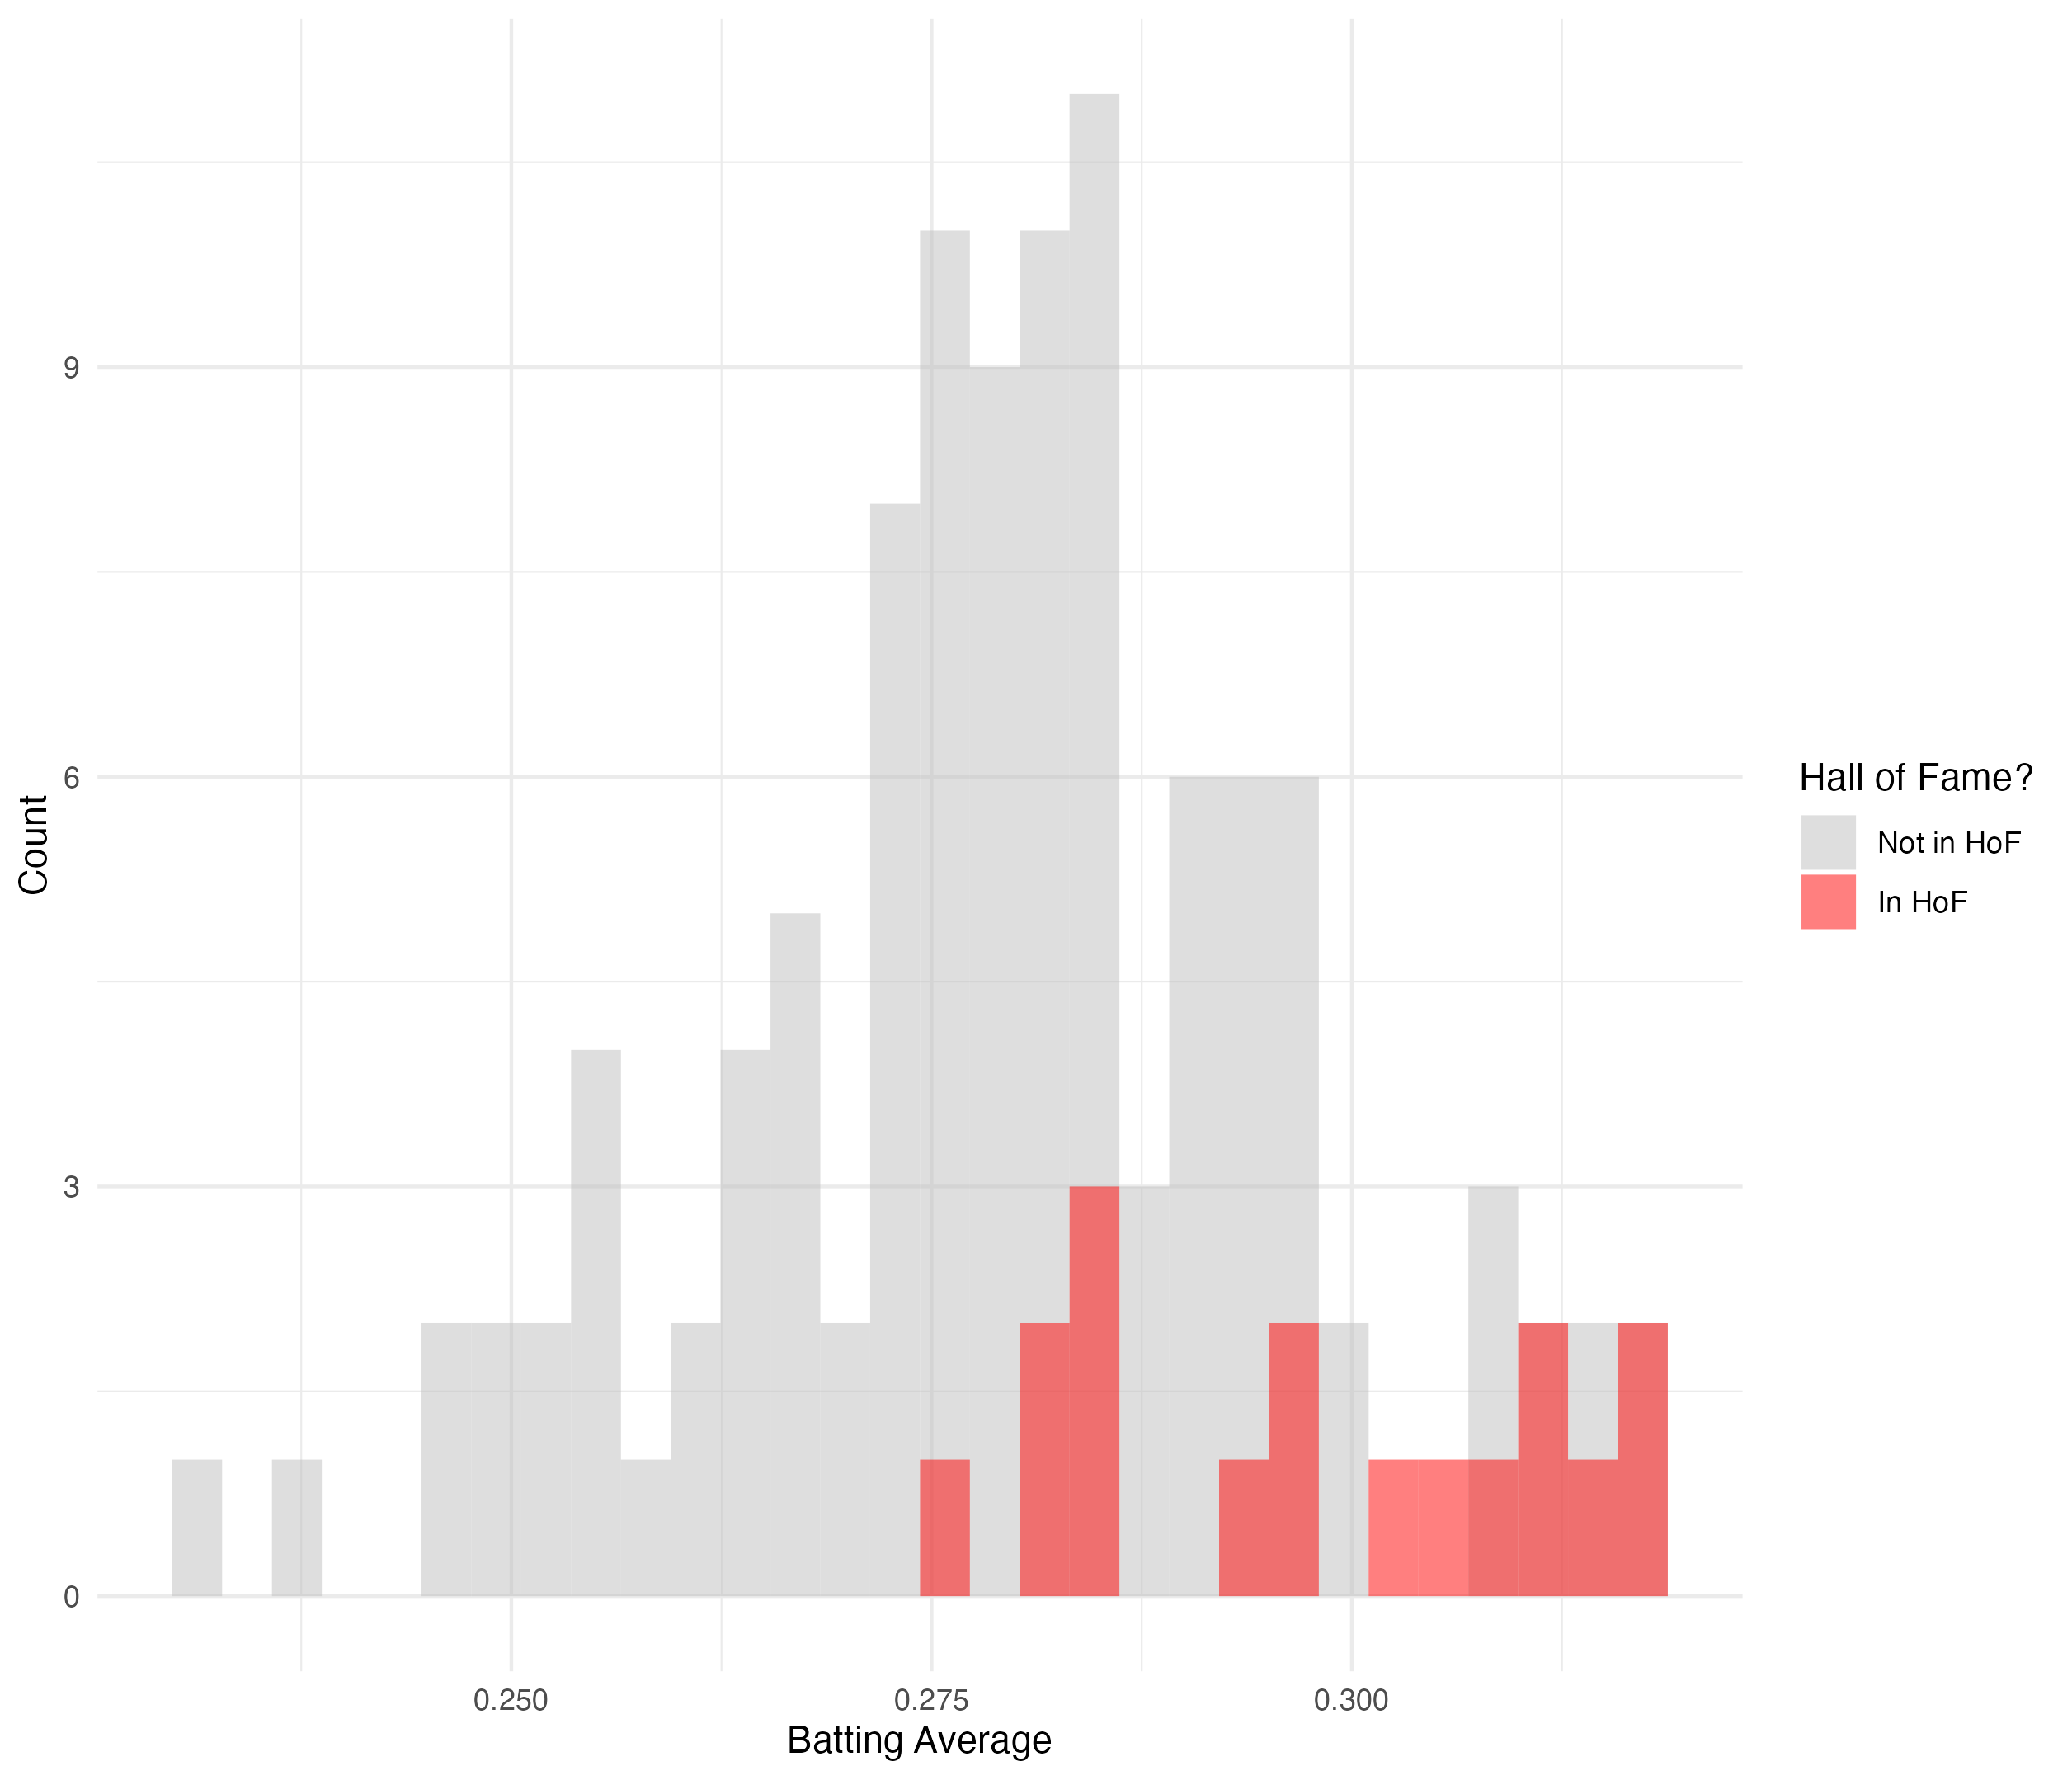
\includegraphics[width=.9\linewidth]{ba_plot.png}
\caption{Layered Histogram of Batting Average}
\label{fig:fig1}
\end{figure}

%----------------------------------------
% Figure 2
%----------------------------------------
\begin{figure}[ht]
\centering
\bigskip{}
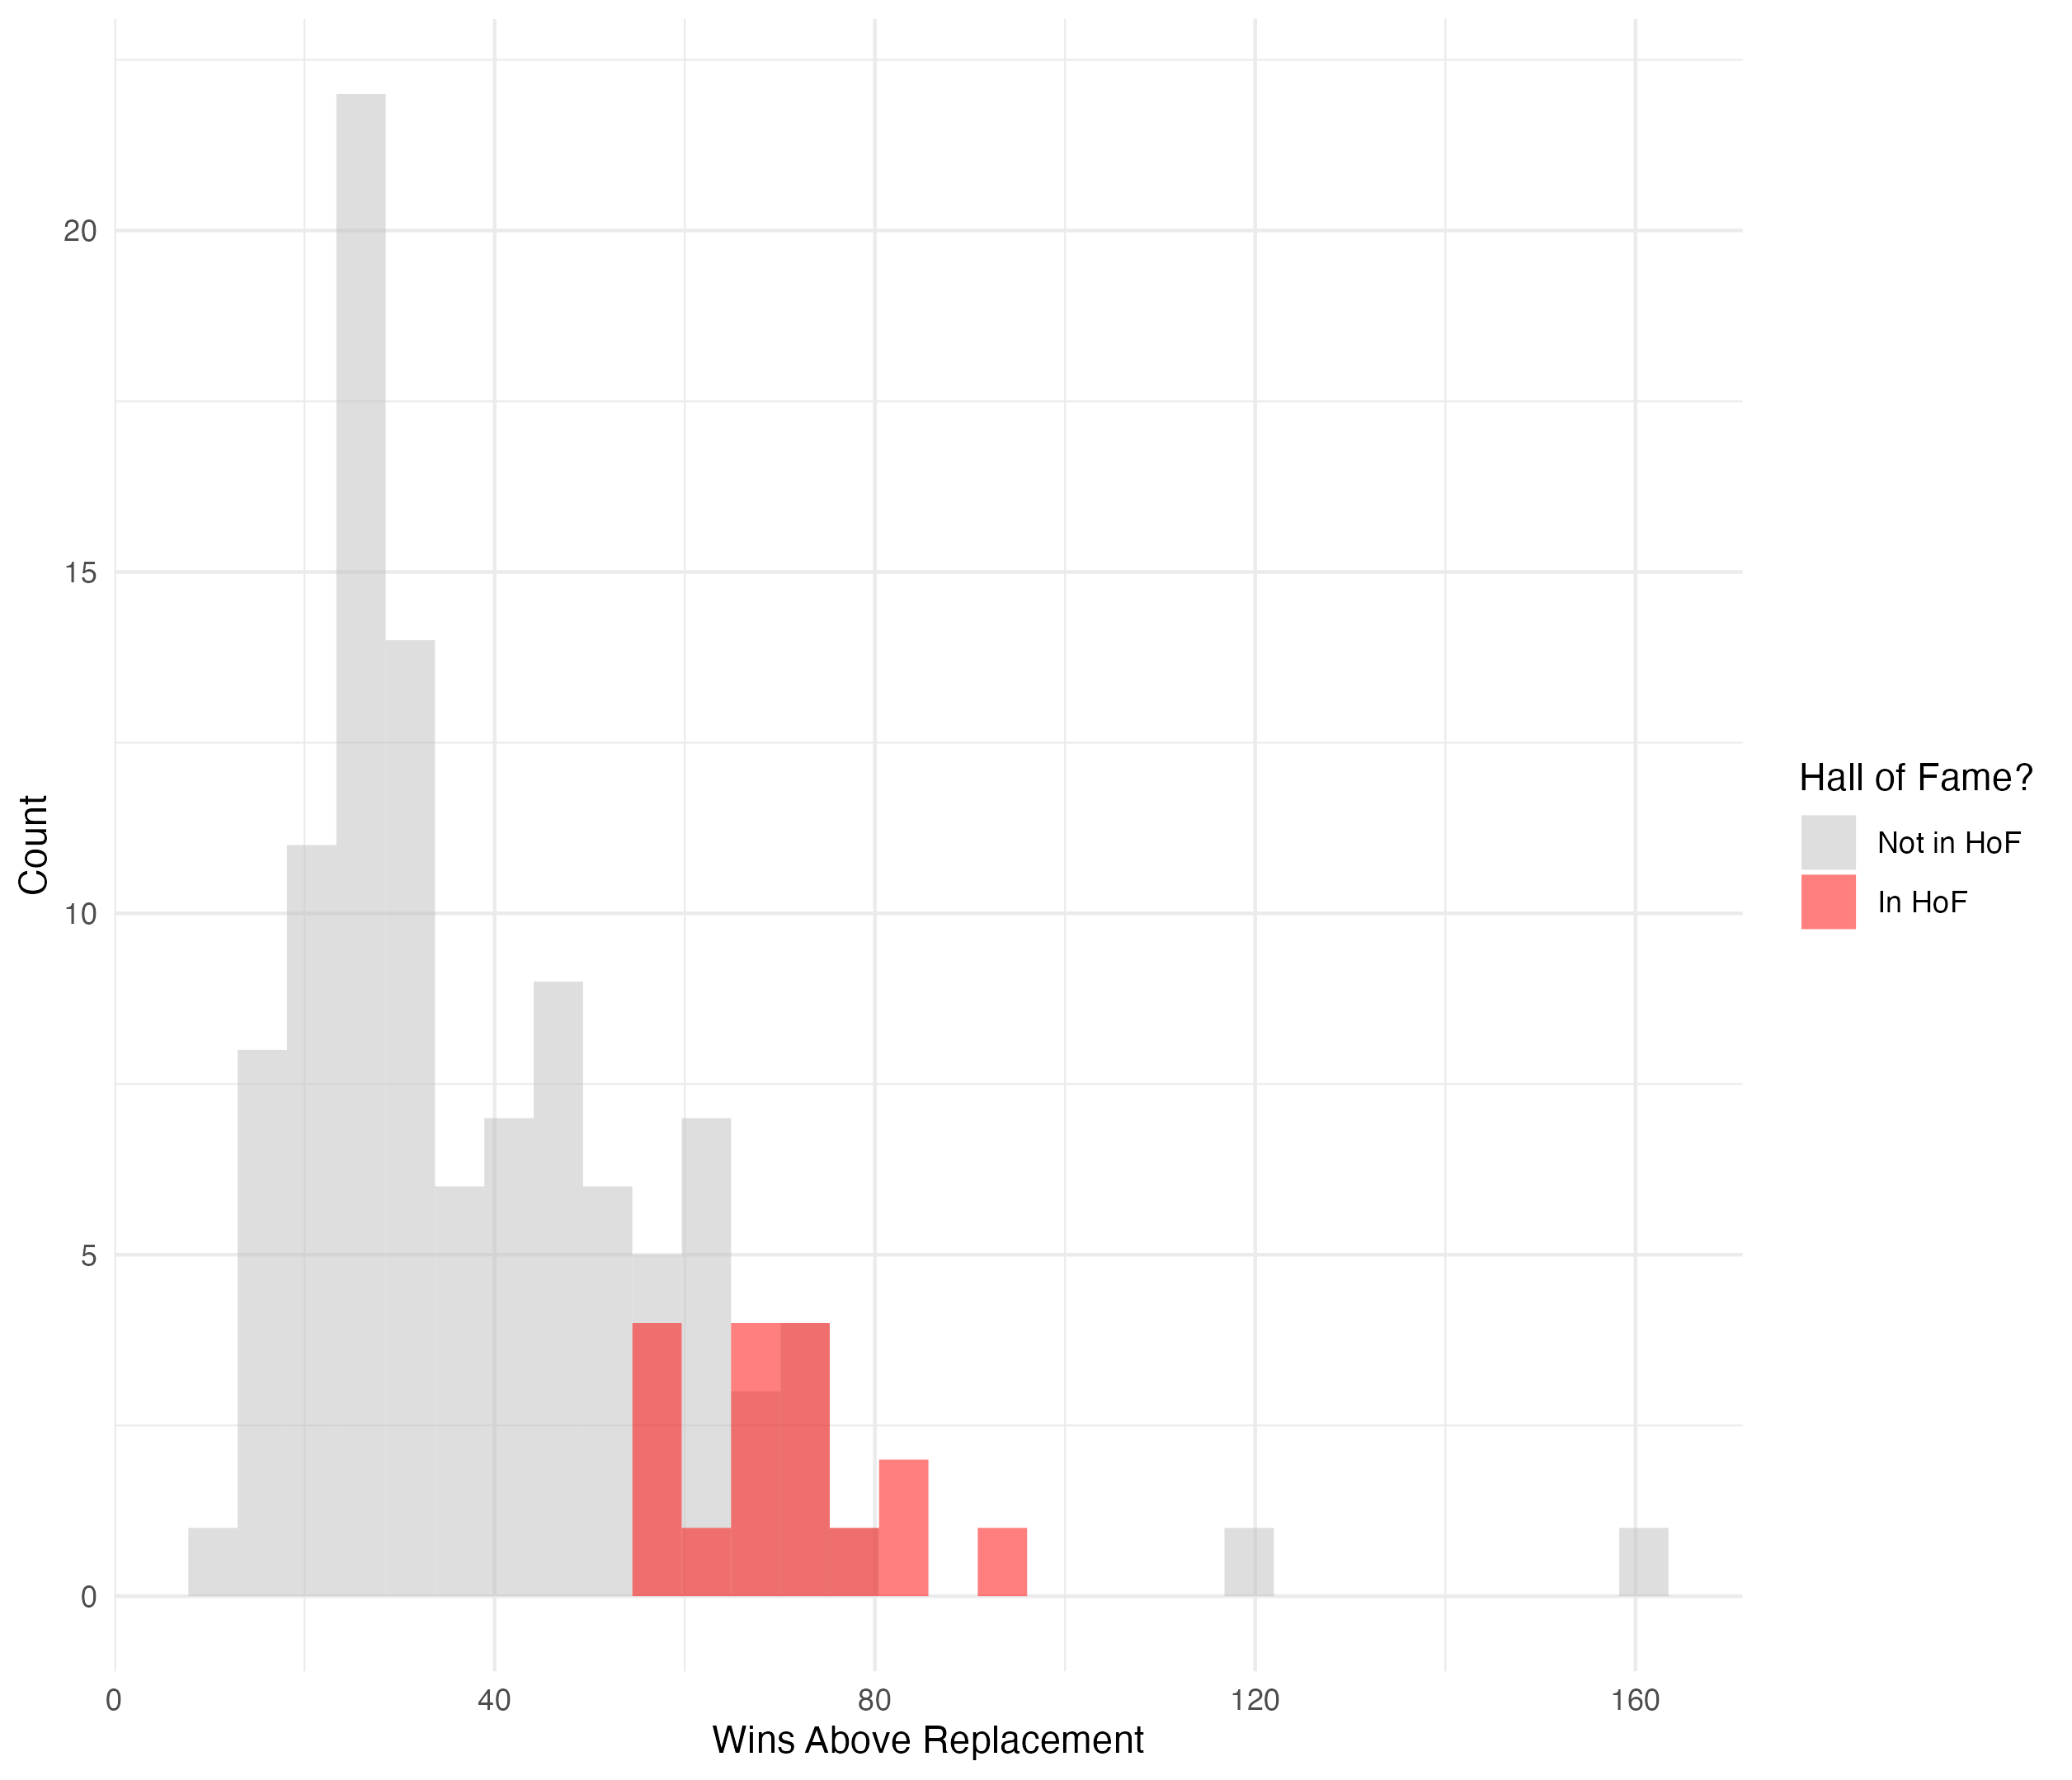
\includegraphics[width=.9\linewidth]{war_plot.png}
\caption{Layered Histogram of Wins Above Replacement}
\label{fig:fig2}
\end{figure}

%----------------------------------------
% Figure 3
%----------------------------------------
\begin{figure}[ht]
\centering
\bigskip{}
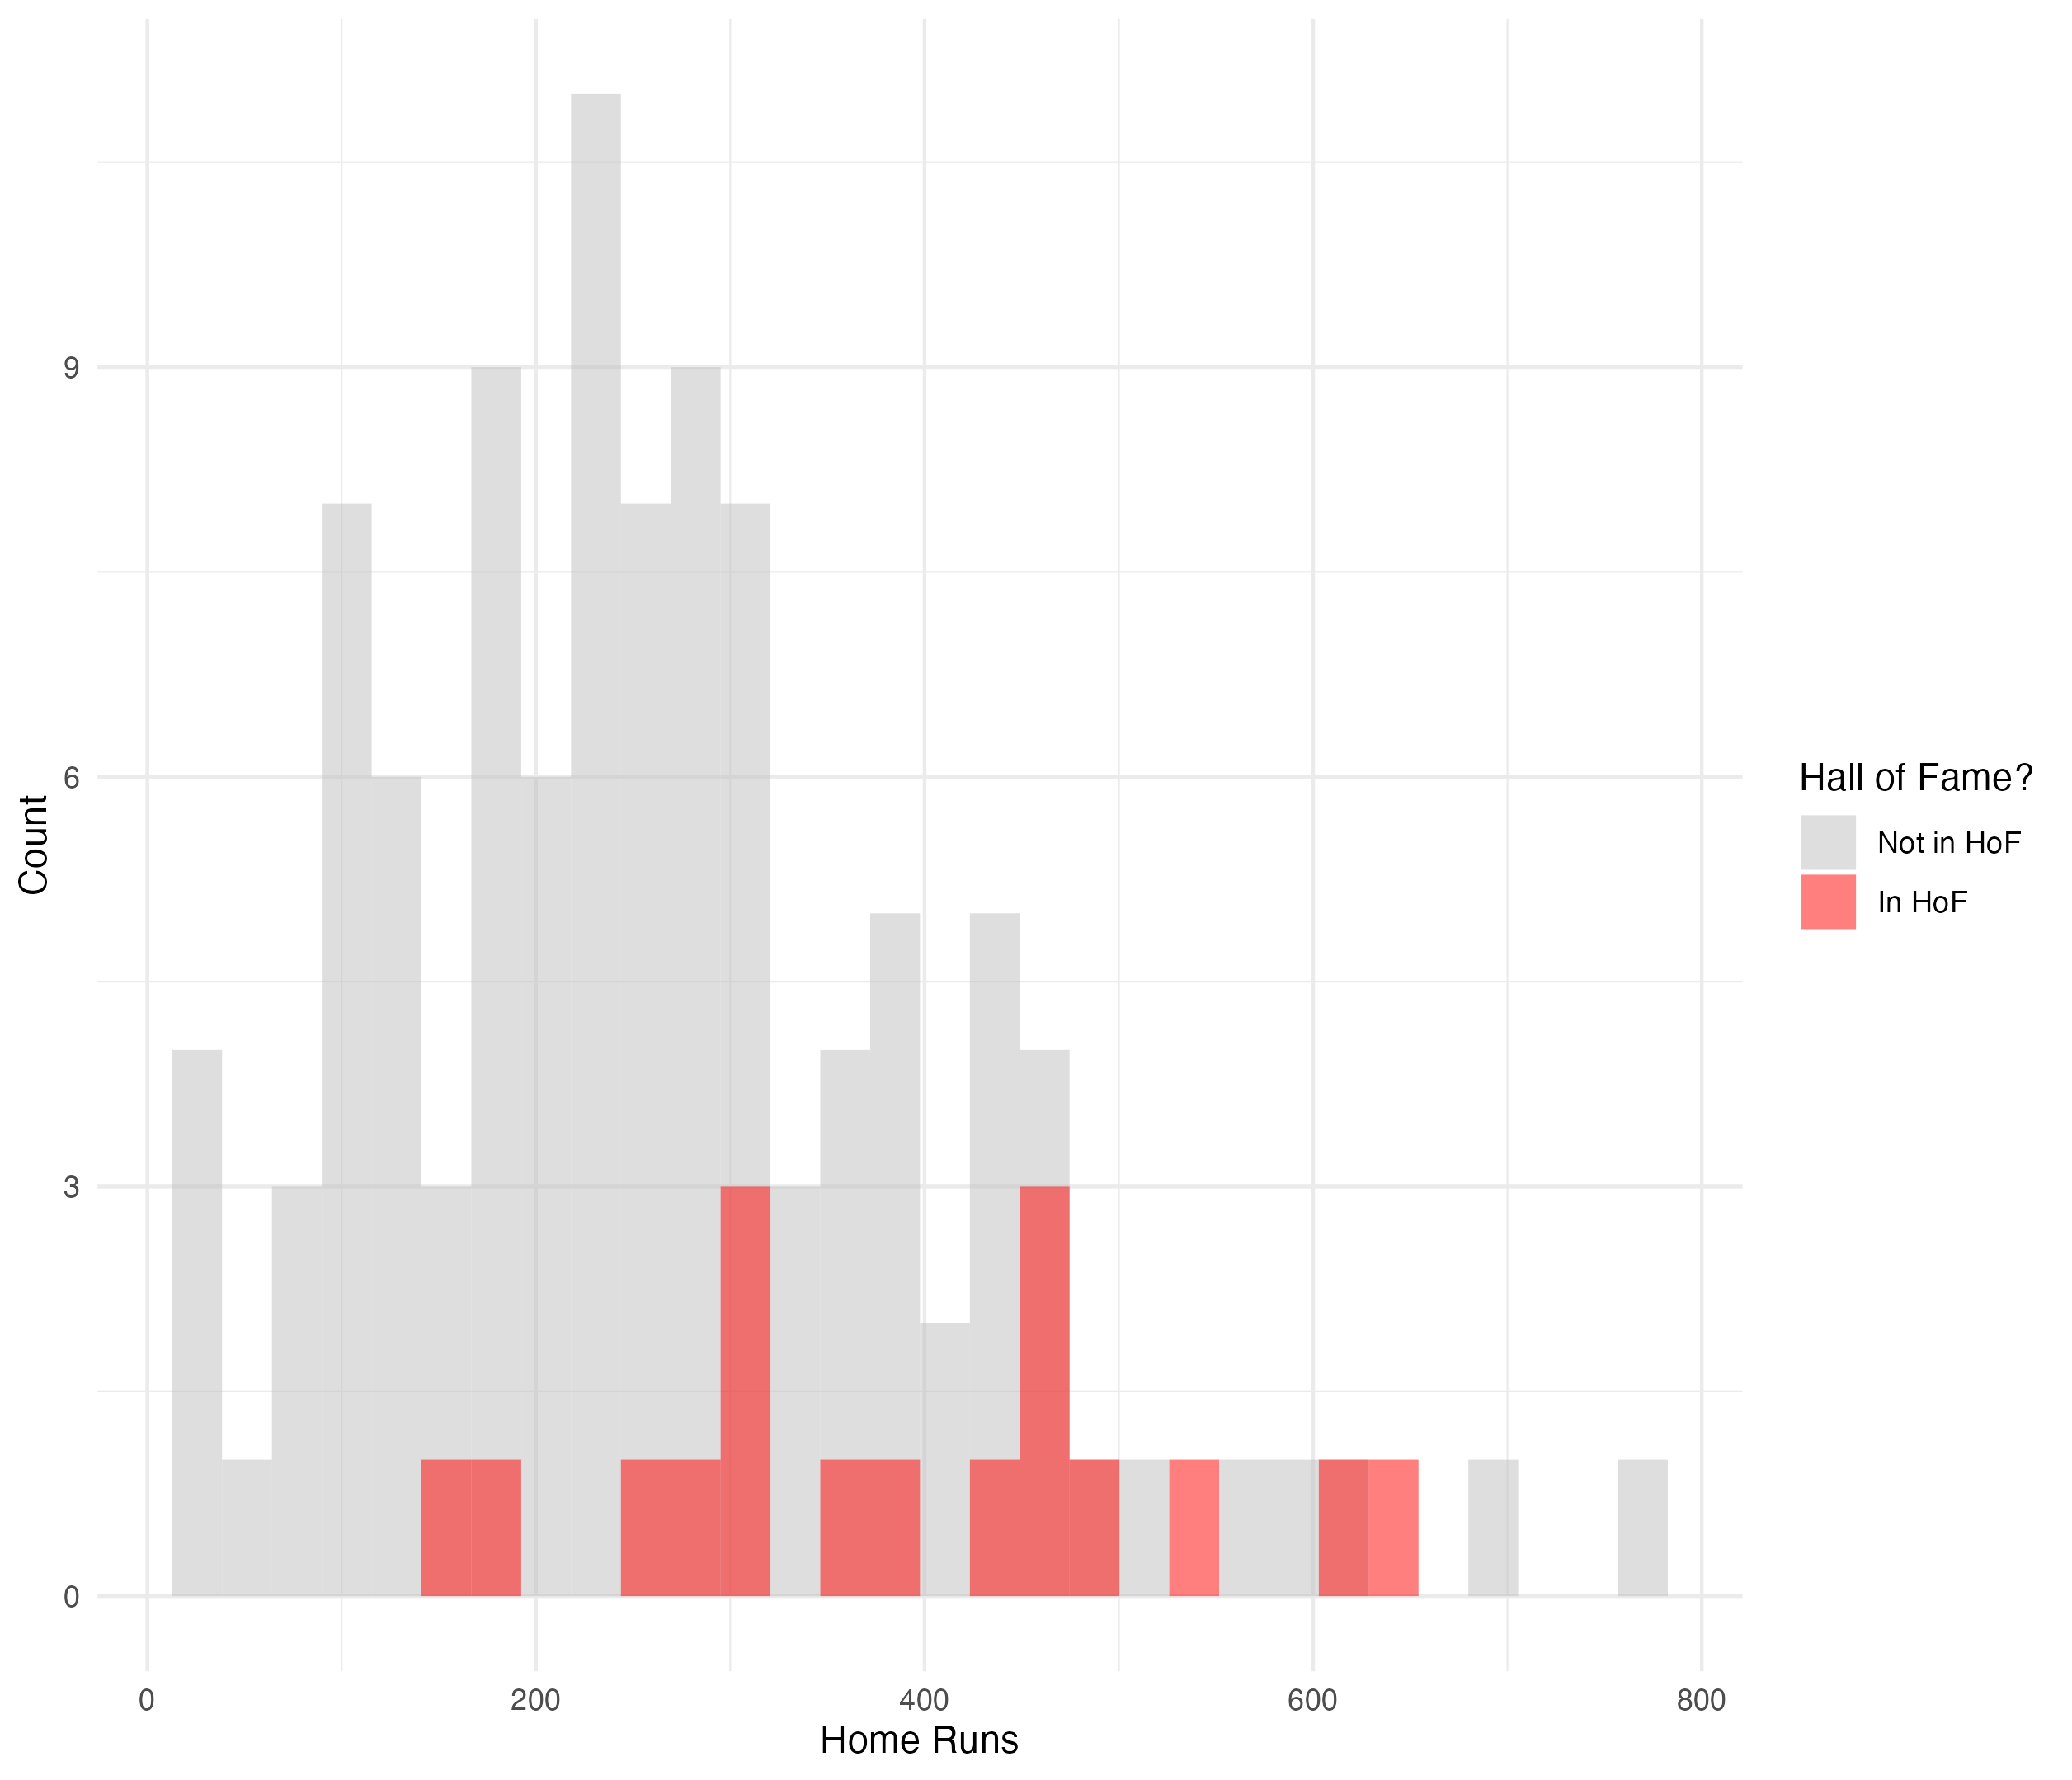
\includegraphics[width=.9\linewidth]{hr_plot.png}
\caption{Layered Histogram of Home Runs}
\label{fig:fig3}
\end{figure}

%----------------------------------------
% Table 1
%----------------------------------------
\begin{table}[ht]
\caption{Summary Statistics of Predictor Variables}
\vspace{10pt}
\centering
\begin{tabular}{rrrrrrr}
  \hline
 & Min. & Q1 & Median & Mean & Q3 & Std.Dev. \\ 
  \hline
HOFm & 4.00 & 35.50 & 80.00 & 92.55 & 120.50 & 70.51 \\ 
  HOFs & 11.00 & 23.50 & 34.00 & 36.12 & 46.00 & 15.61 \\ 
  Yrs & 10.00 & 14.00 & 15.00 & 15.89 & 17.50 & 3.03 \\ 
  WAR & 12.30 & 25.80 & 38.80 & 43.68 & 59.50 & 23.24 \\ 
  WAR7 & 12.90 & 23.75 & 31.10 & 32.15 & 41.55 & 10.90 \\ 
  JAWS & 13.50 & 24.70 & 35.50 & 37.92 & 51.05 & 16.89 \\ 
  Jpos & 44.30 & 53.40 & 55.50 & 54.49 & 56.70 & 3.61 \\ 
  Batter\_G & 904.00 & 1593.00 & 1912.00 & 1920.88 & 2182.50 & 431.78 \\ 
  AB & 3402.00 & 5642.50 & 6930.00 & 6952.28 & 8059.50 & 1673.96 \\ 
  R & 434.00 & 812.50 & 1055.00 & 1086.14 & 1273.50 & 332.03 \\ 
  Batter\_H & 1012.00 & 1524.50 & 2029.00 & 1973.68 & 2334.00 & 528.21 \\ 
  Batter\_HR & 18.00 & 180.00 & 267.00 & 284.21 & 379.50 & 148.48 \\ 
  RBI & 371.00 & 780.00 & 1003.00 & 1069.05 & 1321.50 & 367.31 \\ 
  SB & 5.00 & 29.50 & 94.00 & 146.70 & 205.50 & 158.53 \\ 
  Batter\_BB & 180.00 & 543.50 & 737.00 & 813.14 & 968.50 & 362.33 \\ 
  BA & 0.23 & 0.27 & 0.28 & 0.28 & 0.29 & 0.02 \\ 
  OBP & 0.30 & 0.34 & 0.36 & 0.36 & 0.38 & 0.03 \\ 
  SLG & 0.34 & 0.43 & 0.47 & 0.47 & 0.51 & 0.05 \\ 
  OPS & 0.67 & 0.78 & 0.82 & 0.83 & 0.88 & 0.07 \\ 
  OPS+ & 75.00 & 104.00 & 117.00 & 117.83 & 130.50 & 18.54 \\ 
   \hline
\end{tabular}
\end{table}
%----------------------------------------
% Table 2
%----------------------------------------
\begin{table}[ht]
\caption{Confusion Matrix for Predictions on Test Data}
\vspace{10pt}
\centering
\begin{tabular}{rrr}
  \hline
 & Truth 0 & Truth 1 \\ 
  \hline
Prediction 0 & 30.00 & 4.00 \\ 
  Prediction 1 & 2.00 & 2.00 \\ 
   \hline
\end{tabular}
\end{table}


\end{document}
